\documentclass[12pt, letterpaper]{article}
\usepackage[margin=1.0in]{geometry}
\usepackage{amsmath}
\usepackage{amssymb}
\usepackage{fancyhdr}
\usepackage{pgfplots}
\usepackage{physics}
\usepackage{wrapfig}
\pgfplotsset{compat=1.16}



\title{Classical Mechanics PS1}
\author{Joe Crowley}
\date{October 2020}

\pagestyle{fancy}
\renewcommand{\headrulewidth}{0pt}
\renewcommand{\footrulewidth}{0pt}

\fancyhf{}
\rhead{
Joe Crowley \\
Physics 205 \\
Problem Set 1
}
\rfoot{Page \thepage}

\begin{document}


\section{GPS Exercise 12}
\textit{The escape velocity of a particle on Earth is the minimum velocity required at Earth's surface in order that the particle can escape from Earth's gravitational field. Neglecting the resistance of the atmosphere, the system is conservative. From the conservation theorem0 for potential plus kinetic energy, show that the escape velocity for Earth, Ignoring the presence of the Moon, is $11.2 \mathrm{km} / \mathrm{s}$.}

$$
    \frac{l}{2} m v_{esc}^{2}= \left | U_{esc} \right|
$$
$$
\left|U_{esc}\right|=\int_{R_{Earth}}^{\infty} \vec{F} \cdot \vec{\mathrm{d} r}
$$
$$
=\int_{R_{Earth}}^{\infty} \frac{G m_{Earth} m}{r^{2}} \mathrm{d} r
$$
$$
=G m_{Earth} m\left(-\left.\frac{1}{r}\right|_{R_{Earth}} ^{\infty}\right)
$$
$$
\frac{1}{2} m v_{esc}^{2}=\frac{G m_{Earth} m}{R_{Earth}}
$$
$$
\boxed{V_{esc}=\sqrt{\frac{2 G m_{Earth}}{R_{Earth}}}}
$$


\section{GPS Exercise 14}
\textit{Two points of mass $m$ are joined by a rigid weightless rod of length $l$, the center of which is constrained to move on a circle of radius $a$. Express the kinetic energy in generalızed coordinates.}

Note that there are 2 degrees of freedom if the rod is confined to the x-y plane.
\begin{figure}[h!]
    \centering
    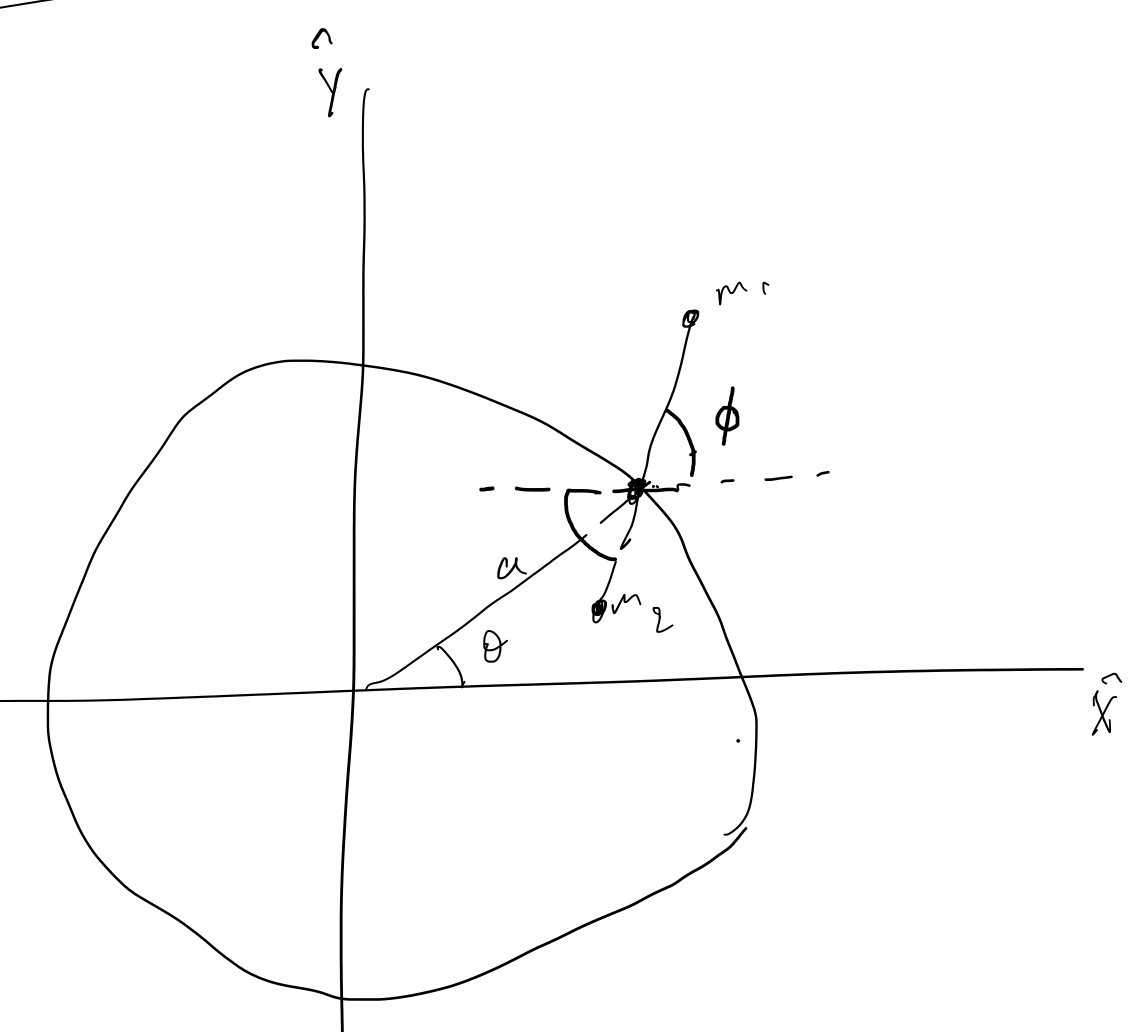
\includegraphics[width=0.4\textwidth]{figures/p14_fig1.png}
\end{figure}

The position vectors for each mass in terms of the generalized coordinates are:
$$
\vec{r}_{1}\left(\theta, \phi\right) =
\left(\begin{array}{c}
a \cos (\theta)+\frac{1}{2} l \cos (\phi) \\
a \sin (\theta)+\frac{1}{2} l \sin (\phi)
\end{array}\right)
$$

$$
\vec{r}_{2}\left(\theta, \phi\right) = \left(\begin{array}{l}
a \cos (\theta)-\frac{1}{2} l \cos (\phi) \\
a \sin (\theta)-\frac{1}{2} l \sin (\phi)
\end{array}\right)
$$


$$
\left| \dot{\vec{r}}_{1}\left(\theta, \phi\right) \right|^2= 
\left(-a \dot{\theta} \sin (\theta)-\frac{1}{2} l \dot{\phi} \sin (\phi)\right)^{2}+\left(a \dot{\theta} \cos (\theta)+\frac{1}{2} l \dot{\phi} \cos (\phi)\right)^{2}
$$
$$
\left| \dot{\vec{r}}_{2}\left(\theta, \phi\right) \right|^2= 
\left(\frac{1}{2} l \dot{\phi} \sin (\phi)-a \dot{\theta} \sin (\theta)\right)^{2}+\left(a \dot{\theta} \cos (\theta)-\frac{1}{2} l \dot{\phi} \cos (\phi)\right)^{2}
$$

$$\left| \dot{\vec{r}}_{1}\left(\theta, \phi\right) \right|^2+\left| \dot{\vec{r}}_{2}\left(\theta, \phi\right) \right|^2 = 
2 a^{2} \dot{\theta}^{2} \sin ^{2}(\theta)+2 a^{2} \dot{\theta}^{2} \cos ^{2}(\theta)+\frac{1}{2} l^{2} \dot{\phi}^{2} \sin ^{2}(\phi)+\frac{1}{2} l^{2} \dot{\phi}^{2} \cos ^{2}(\phi)
$$

$$
=2 a^{2} \dot{\theta}^{2}+\frac{1}{2} l^{2} \dot{\phi}^{2}
$$


$$
\boxed{
T=\frac{1}{2} \sum_{i} m_{i}\left|\dot{\vec{r}}_{i}\right|^{2} = a^{2} m \dot{\theta}^{2}+\frac{1}{4} l^{2} m \dot{\phi}^{2}
}
$$

\section{GPS Exercise 21}
\textit{Two mass points of mass $m_{1}$ and $m_{2}$ are connected by a string passing through a hole in a smooth table so that $m_{1}$ rests on the table surface and $m_{2}$ hangs suspended. Assuming $m_{2}$ moves only in a vertical line. what are the generalized coordinates for the system? Write the Lagrange equations for the system and, if possible, discuss the physical significance any of them might have. Reduce the problem to a single second-order differential equation and obtain a first integral of the equation. What is its physical significance? (Consider the motion only until $m_{1}$ reaches the hole.)}


\begin{figure}[h!]
    \centering
    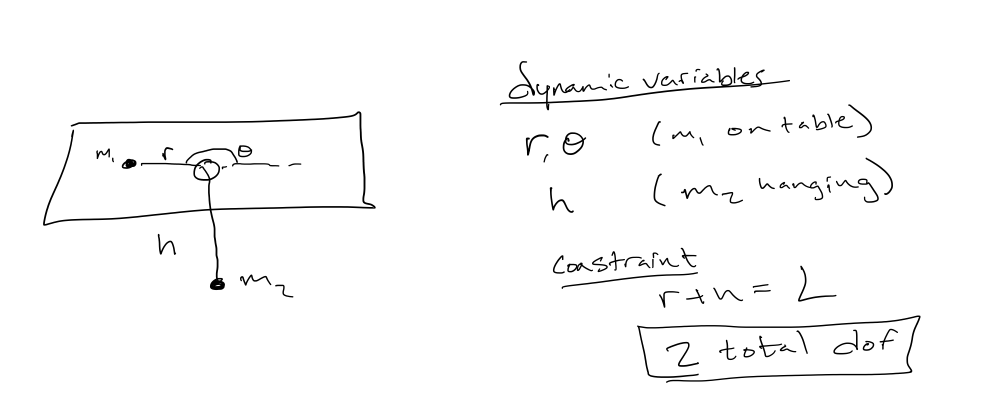
\includegraphics[width=0.8\textwidth]{figures/p21_fig1.png}
\end{figure}

$$
T_{1}=\frac{1}{2} m_{1} \dot r^{2}+\frac{1}{2} m_2 r^{2} \dot{\theta}^{2}
$$

$$
T_{2}=\frac{1}{2} m_{2} \dot{r}^{2}
$$
$$
U_{1}=0
$$
$$
U_{2}=-m_2 \mathrm{g}(L-r)
$$

$$
\mathrm{L}=\sum T_{i}-{U_{i}}
$$
$$
\boxed{
\mathrm{L}=\frac{1}{2} m_1 \dot{r}^{2}+\frac{1}{2} m_1 r^{2} \dot{\theta}^{2}+\frac{1}{2} m_2 \dot{r}^{2}+m_{2} g(L-r)
}
$$

$$
\frac{\partial \mathrm{L}}{\partial r}=\frac{d}{d t}\left(\frac{\partial \mathrm{L}}{\partial \dot{r}}\right)
$$
$$
m_{1} \dot r \dot{\theta}^{2}-m_{2} g=\left(m_1+m_{2}\right) \ddot{r}
$$

$$
\frac{\partial \mathrm{L}}{\partial \theta}=\frac{d}{d t}\left(\frac{\partial \mathrm{L}}{\partial \dot{\theta}}\right)
$$

$$
\frac{\partial L}{\partial \dot{\theta}}=\text { constant }
$$
This equation leads to conservation of angular momentum!
$$
\dot{\theta}=\frac{p_{\theta}}{m_{1} r^{2}}
$$

$$
\boxed{
\left(m_{1}+m_{2}\right) \ddot{r}=\frac{p_{\theta}^{2}}{m_{1} r^{3}}-m_{2} g
}
$$
Now, to do a First Integral multiply both sides by $\dot r$,
$$
\left(m_{1}+m_{2}\right) \ddot{r} \dot{r}+\frac{p_{\theta}^{2}}{m_{1}} \frac{\dot{r}}{r^{3}}+m_{2} g \dot{r}=0,
$$
And integrate:
$$
\boxed{
\frac{1}{2}\left(m_{1}+m_{2}\right) \dot{r}^{2}-\frac{p_{\theta}^{2}}{2 m_{1} r^{2}}+m_{2} g r= constant}
$$
The First Integral of these Equations of Motion is a statement of the conservation of energy!
\end{document}
